% !TEX encoding = UTF-8 Unicode
% ÄÖÜ ß äöü

The aim of this project was to design an interactive environment on a tablet computer 
that allows the user to learn simple facts about the formalism of propositional logic 
and standard transformations of Boolean functions. 
The environment was meant to be self-explanatory. 

The core of this concept builds on tutorials with exercises 
and a playground where the learned knowledge can be used in different modes. 
A glossary of terms and a formula calculator (BoolTool) to check formulas will support the user in their learning.

\section{Tutorials}

Ny$\bar{a}$ya for iPad covers syntax and semantics of propositional logic, 
but only some basic rules of natural deduction. 
It introduces normal forms, truth tables and binary decision diagrams 
as different but equivalent representations of boolean functions.

The structure of the tutorials and the content of the exercises are heavily based on the according sections of the book  
{\em Logic in Computer Science} \cite{Huth:2004:LCS:975331} by M.~Huth and M.~Ryan.
Additional content is taken from the lecture {\em Logic} \cite{Middeldorp:2012:LICS} by {A. Middeldorp}

\begin{table}[htdp]
\begin{center}
\begin{lstlisting}[mathescape,firstnumber=5]
	<array> 		<!-- root with title and sections -->
	<string>Tutorials</string> 					<!-- title -->
	<array>			<!-- section with title and tutorials-->
		<string>Introduction</string> 				<!-- section title -->
		<array>		<!-- tutorial with title and id -->
			<string>Motivation</string> 	<!-- tutorial title -->
			<string>101</string> 						<!-- tutorial id -->
		</array>
		$\square$
\end{lstlisting}
\caption{Tutorial.plist – configuration file for all tutorials}
\label{tab:TUTORIALPLIST}
\end{center}
\end{table}%

General and specific configurations for the tutorials and additional content for the exercises 
are stored in simple property lists\footnote{
\href{http://www.apple.com/DTDs/PropertyList-1.0.dtd}{http://www.apple.com/DTDs/PropertyList-1.0.dtd}
\tabref{tab:PLISTDTD}. }, which are xml-files with basic data types, that can be easily read and interpreted by different programs.
The file “Tutorials.plist” \tabref{tab:TUTORIALPLIST} provides the basic data about available tutorial sections and tutorial titles 
to build a navigation menu programmatically.

Every tutorial includes a teaching part with examples (html files with utf8 encoding) 
and interactive knowledge checker with exercises, 
where the user gets immediate feedback. 
Every interactive part will present some instructions to master the tasks.

\subsection{Introduction}

The first tutorial section with four tutorials 
(\hyperref[tut:101]{101}, 
\hyperref[tut:102]{102}, 
\hyperref[tut:103]{103},
\hyperref[tut:104]{104}
) 
gives an informal overview to modeling, 
i.e. the translation from sentences in natural language to more formal sentences. 

%\begin{table}[htdp]
%\begin{center}
%\begin{lstlisting}[mathescape]
%<?xml version="1.0" encoding="UTF-8"?>
%<!DOCTYPE plist PUBLIC "-//Apple//DTD PLIST 1.0//EN" 
%	"http://www.apple.com/DTDs/PropertyList-1.0.dtd">
%<plist version="1.0">
%	$\square$	
%</plist>
%\end{lstlisting}%
%\caption{Structure of a simple property list}
%\label{tab:PLISTHEAD}
%\end{center}
%\end{table}


The content file “QA1.plist” \tabref{tab:QA1} contains
an array (starts at line 5) 
of arrays that include sentences and sample solutions 
(the first exercise starts at line 6). 
The first string is the sample sentence (at line 7), 
which must be analyzed by the user
and the following entries are sample solutions for different exercises. 

\begin{table}[htdp]
\begin{center}
\begin{lstlisting}[firstnumber=5]
	<array>
		<array> 
			<string>If the barmoter falls, then it will rain.</string>
			<string>if p then q</string>
			<string>the barometer falls; it will rain</string>
			<string>p $\rightarrow$ q</string>
		</array>
		$\square$
\end{lstlisting}
\caption{QA1.plist – content file for the first three tutorials}
\label{tab:QA1PLIST}
\end{center}
\end{table}%

Each tutorial has its own configuration file \tabref{tab:101PLIST}
with a dictionary that
 describes the task and defines the index of the sample solution,
 with which the user's answer will be compared with some tolerance.

\begin{table}[htdp]
\begin{center}
\begin{lstlisting}[firstnumber=5]
<dict>
	<key>questionLabelText</key>
	<string>Guess the structure …</string>
	<key>answerLabelText</key>
 	<string>Use … </string>
 	<key>solutionLabelText</key>
 	<string>Sample solution</string>
 	<key>questionsFile</key>
 	<string>QA1</string>
 	<key>solutionIndex</key>
 	<integer>1</integer>
</dict>
\end{lstlisting}
\caption{101.plist – configuration file for the first exercise}
\label{tab:101PLIST}
\end{center}
\end{table}%



\begin{verbatim}
\end{verbatim}

\subsubsection{Motivation – the composite structure of sentences}
\label{tut:101}

(101) The aim of logic in general is to reason about situations.\cite{Huth:2004:LCS:975331} 
The common structure of two composite sentences in natural language 
is reduced to “If p and not q, then r. Not r. p. Therefore, q“. 
If the reasoning is correct, the user can it use in both situations. 

In the interactive part the user has to guess the structure of composite sentences in natural language. 
For he sample sentence 
\verb+‘If the barometer falls,+ \verb+then it will rain’+ 
from line 7 of \verb+QA1.plist+ (\tabref{tab:QA1PLIST})
the user has to answer with line 8 
\verb+‘if p then q’+, (solution index is defined as 1 in \verb+101.plist+, see \tabref{tab:101PLIST}).

\subsubsection{Propositions – declarative sentences}
\label{tut:102}

(102) The concept of propositions – declarative sentences – 
as indivisible building blocks of propositional logic 
is explained in more detail. Some counterexamples are presented 
and the ambiguity of natural language is demonstrated.

The user has to find the propositions in composite sentences. 
For he sample sentence from \verb+QA1.plist+ (\tabref{tab:QA1PLIST})
the user has to answer with line 9 
\verb+‘the barometer falls; it will rain’+, (solution index is defined as 2 in \verb+102.plist+).


\subsubsection{Symbols – emphasize the structure}
\label{tut:103}

(103) The symbols to replace “if then”, “not”, “and” and “or” are introduced. 

Now the user should transform the sentences from the first tutorial into pure propositional formulas. 
For he sample sentence from \verb+QA1.plist+ (\tabref{tab:QA1PLIST})
the user has to answer with \verb+‘p+ $\rightarrow$ \verb+q’+ (solution index is defined as 3 in \verb+103.plist+).

\subsubsection{Limits}
\label{tut:104}

(104) Not every situation can be transformed into a formula in propositional logic. 
This tutorial has no interactive part.

\subsection{Syntax}

After the informal introduction into the atoms and connectives of propositional logic, 
the formal aspects of propositional logic will be introduced to the user.

The content of the exercises will be generated by the app and the user's solution will be checked without tolerance.


\subsubsection{Well formed formulas}
\label{tut:201}

(201) The concept of well formed formulas is explained. 

\begin{table}[htdp]
\begin{center}
\begin{tabular}{rcccccccccc}
$P$	&$::=$	&$p$ 	
	&|		& $(\neg P)$ 
	&|		&  $(P \wedge P)$ 
	&|		&  $(P \vee P)$ 
	&|		&  $(P \rightarrow P)$ \\
\end{tabular}
\caption{grammer with mandatory parenthesis}
\label{tab:BNFGRPA}
\end{center}
\end{table}

The user has to build simple well formed formulas: 
“a conjcuntion”, “an disjunction of an negation”, “a negation of an implication” and so on.
They have to use parenthesis.

\subsubsection{Conventions for your convenience}
\label{tut:202}

(202) Precedence of connectives is introduced. 
The user has to rewrite formulas 
to save some parenthesis.

\begin{table}[htdp]
\begin{center}
\begin{tabular}{rcccl}
$P$		&$::=$ & $D$ &|& $P \rightarrow D$\\
$D$		&$::=$ & $C$ &|& $C \vee D$			\\
$C$		&$::=$ & $N$ &|& $N \wedge C$ 		\\
$N$		&$::=$ & $T$ &|& $\neg N$ 			\\
$T$		&$::=$ & $p$ &|& $(P)$
\end{tabular}
\caption{grammar with precedences}
\label{tab:BNFGRPR}
\end{center}
\end{table}

%\begin{table}[htdp]
%\begin{center}
%\begin{tabular}{rcl}
%P		&$::=$ & D [ $\rightarrow$ P ]\\
%D		&$::=$ & C \{ $\vee$ C \}\\
%C		&$::=$ & N  \{ $\wedge$ N \} \\
%N		&$::=$ & $\neg$N | p | (P) \\
%\end{tabular}
%\caption{EBNF Grammar (with precedences)}
%\label{tab:BNF}
%\end{center}
%\end{table}

\subsubsection{Subformulas}
\label{tut:203}

(203) Subformulas (starting from atoms) are use to build bigger formulas. Big formulas are build from many sub formulas.
The user have to find all sub formulas of simple composite formulas.

\subsubsection{Syntax Trees}
\label{tut:204}

(204) This tutorial explains how to draw an syntax tree (starting with atoms)
The user has to draw the syntax tree of simple formulas. They has to pay attention to the precedence of connectives.

\subsubsection{Additional symbols – Top and Bottom}
\label{tut:205}

(205) The tutorial 
introduces symbols “$\top$” (top) and “$ \bot$” (bottom)
as abbreviations of conjunctions and disjunctions 
of formulas with their negation (tautologies and contradictions, \tabref{tab:TopBottom}).
The user has to rewrite some formulas replacing contradictions and tautologies with top and bottom.

\begin{table}[htdp]
\begin{center}
\begin{tabular}{c|c|c|c}
$\neg P \vee P$&$P \vee \neg P$  & $\neg P \wedge P$ & $P \wedge \neg P$ \\
\hline
$\top$ & $\top$ & $ \bot$&$ \bot$\\
\end{tabular}
\caption{tautologies and contradictions}
\label{tab:TopBottom}
\end{center}
\end{table}%

\subsubsection{Simplifying formulas – basic natural deduction rules}
\label{tut:206}

(206) The tutorial teaches the simplifying of conjunctions and disjunctions with top, bottom and/or the same sub formulas.



\begin{table}[htdp]
\begin{center}
\begin{tabular}{c|c|c|c|c}
$\neg \neg P$ & $P \vee P$ & $P \wedge P$ & $P \vee Q$ & $P \wedge Q$\\
\hline
$P$ & $P$ & $P$ & $Q \vee P$ & $Q \wedge P$\\
\end{tabular}
\caption{basic rules}
\label{tab:BasicRules}
\end{center}
\end{table}%

The user has to rewrite some formulas eleminating 
top, bottom, double negations, conjunctions and disjunctions 
by using rules from 
\tabref{tab:TopBottom} and \tabref{tab:BasicRules}.

\subsubsection{Conjunctive Normal Form} 
\label{tut:207}
(207) The syntax of formulas in conjunctive normal form is introduced (\tabref{tab:CNF}) and explained.
It is shown that some formulas in cnf can be simplified to top.
\begin{table}[htdp]
\begin{center}
\begin{tabular}{rcccl}
$C$	&$::=$ & $(D)$ 	&$|$ & $(D) \wedge C$\\
$D$	&$::=$ & $L$ 	&$|$ & $L \vee D$\\
$L$	&$::=$ & $p$ 	&$|$ & $\neg p$ 
\end{tabular}
\caption{grammar for conjunctive normal form}
\label{tab:CNF}
\end{center}
\end{table}

The user has to guess if a presented formula is in conjunctive normal form
and if it can be simplified to top ($\top$).


\subsubsection{Disjunctive Normal Form} 
\label{tut:208}
(208) The syntax of formulas in disjunctive normal form is introduced (\tabref{tab:DNF}) and explained.
It is shown that some formulas in dnf can be simplified to bottom.
\begin{table}[htdp]
\begin{center}
\begin{tabular}{rcccl}
$D$	&$::=$ & $C$ 	&$|$ & $C \;\vee D$\\
$C$	&$::=$ & $L$ 	&$|$ & $L \wedge D$\\
$L$	&$::=$ & $p$ 	&$|$ & $\neg p$
\end{tabular}
\caption{grammar for disjunctive normal form}
\label{tab:DNF}
\end{center}
\end{table}

The user has to guess if a presented formula is in disjunctive normal form
and if it can be simplified to bottom ($\bot$).


\subsection{Semantics}

After the introduction of well formed formulas the meaning of logical connectives is defined.

\subsubsection{Truth assignments and valuation of formulas}
\label{tut:301}
(301)
The truth assignment for atoms $(p,q,r,…)$ is introduced and the valuation of top, bottom, negation, conjunction, disjunction and implication is described.

The user has to guess or calculate the evaluation of a given formula with a given truth assignment of the atoms of the formula.

\subsubsection{Truth tables}
\label{tut:302}
(302)
The concept of truth tables is explained and demonstrated with the basic connectives. 
Subformulas are used to demonstrate the valuation of more complex formulas.

The user has to fill in complete truth tables with a maximum of three atoms.

\subsubsection{Semantic Entailment and Equivalence}
\label{tut:303}
(303)
The user has to guess or calculate if an semantic entailment holds. 



\subsubsection{Satisfiability, Tautologies and Contradictions}
\label{tut:304}
(304)

\subsection{Normal Forms}

The advantages of propositional formula in special shapes will be emphasized.
\hyperref[tut:207]{CNFs} and \hyperref[tut:208]{DNFs} are already defined
in \tabref{tab:CNF} and \tabref{tab:DNF}.
The definitions of implication free form and negation normal form will be provided. 
The algorithm to transform arbitrary propositional formula into specific normal forms will be shown.

\subsubsection{Implication Free Form and Negation Normal Form}
\label{tut:401}
(401)
By removing the rule for $P$ from the grammar in \tabref{tab:BNFGRPR} 
the user gets the grammar for implication free formulas 
(\tabref{tab:BNFGRIFF}). 
By removing the rules for arbitrary negations, the negation normal form is defined
 (\tabref{tab:BNFGRNNF}). 

\begin{table}[htdp]
\begin{center}
\begin{tabular}{rcccl}
$D$		&$::=$ & $C$ &|& $C \vee D$			\\
$C$		&$::=$ & $N$ &|& $N \wedge C$ 		\\
$N$		&$::=$ & $T$ &|& $\neg N$ 			\\
$T$		&$::=$ & $p$ &|& $(P)$
\end{tabular}
\caption{grammar without implication}
\label{tab:BNFGRIFF}
\end{center}
\end{table}

\begin{table}[htdp]
\begin{center}
\begin{tabular}{rcccl}
$D$		&$::=$ & $C$ &|& $C \vee D$			\\
$C$		&$::=$ & $N$ &|& $N \wedge C$ 		\\
$N$		&$::=$ & $(P)$ & | & $p $ | $\neg p$
\end{tabular}
\caption{grammar for negation normal form}
\label{tab:BNFGRNNF}
\end{center}
\end{table}

The user has to guess if a formula is implication free and/or in (negation, conjunctive or disjunctive) normal form.

\subsubsection{Get rid of implications}
\label{tut:402}
(402)
%content is missing
The grammars for NNF, CNF, DNF do not include implications. 
So implications has to be removed from formulas by using equivalence transformations to reach the normal forms. 
It is shown with truth tables that the implication of two sub formulas is semantically equivalent 
to the disjunction of the negation of the first sub formula with the second sub formula (\tabref{tab:ET_IFF}).


\begin{table}[htdp]
\begin{center}
\begin{tabular}{r}
$P \rightarrow Q$ \\ 
————\\
$\neg P \;\vee\; Q$
\end{tabular}
\caption{equivalence transformation to remove implications}
\label{tab:ET_IFF}
\end{center}
\end{table}

The user has to rewrite formulas to an implication free form.
The presented formula may already be implication free.

\subsubsection{Negated atoms only}
\label{tut:403}
(403)
The negations normal form is defined. It is shown that the negation of a conjunction is semantically equivalent to the disjunction of the negations.
and the negation of a disjunction is semantically equivalent to the conjunction of the negations and that
double negations can be eliminated (\tabref{tab:ET_NNF}).

\begin{table}[htdp]
\begin{center}
\begin{tabular}{ccr}
$\neg (P \wedge Q) $&$ \neg (P \vee Q)$&$ \neg \neg P$\\
————— & —————& ———\\
$\neg P \vee \neg Q$&$\neg P \wedge \neg Q$&$P$
\end{tabular}
\caption{equivalence transformations toward negation normal form}
\label{tab:ET_NNF}
\end{center}
\end{table}

The user has to rewrite formulas to a negation normal form.
The presented formula is implication free
but may already be in negation normal form.

\subsubsection{NNF to CNF}
\label{tut:404}
(404)
The user learns the distribution of disjunctions over conjunctions (\tabref{tab:ET_CNF}).

\begin{table}[htdp]
\begin{center}
\begin{tabular}{cc}
$P \vee (Q \wedge R)$ & $(P \wedge Q) \vee R$\\
———————— & ————————\\
$(P\vee Q) \wedge (P\vee R)$ & $(P\vee R) \wedge (Q\vee R)$
\end{tabular}
\caption{equivalence transformations towards conjunctive normal form}
\label{tab:ET_CNF}
\end{center}
\end{table}

The user has to rewrite formulas to a conjunctive normal form.  
The presented formula is in negation normal form 
but may already be in conjunctive normal form.


\subsubsection{NNF to DNF}
\label{tut:405}
(405)
The user learns the distribution of conjunctions over disjunctions (\tabref{tab:ET_CNF}).

\begin{table}[htdp]
\begin{center}
\begin{tabular}{cc}
$P \wedge (Q \vee R)$ 			& $(P \wedge Q) \wedge R$\\
———————— & ————————\\
$(P\wedge Q) \vee (P\wedge Q)$ 	& $(P\wedge R) \vee (Q\wedge R)$
\end{tabular}
\caption{equivalence transformations towards disjunctive normal form}
\label{tab:ET_DNF}
\end{center}
\end{table}

The user has to rewrite formulas to a disjunctive normal form. 
The presented formula is in negation normal form 
but may be already be in disjunctive normal form.

\subsubsection{From general formula to CNF or DNF}
\label{tut:406}
(406)
To combination of the previous techniques to reach a equivalent representation in conjunctive or disjunctive normal form is provided.
The potential exponential growing of the length of these transformations is demonstrated.

The user has to rewrite formulas to a conjunctive or disjunctive normal form.
The presented formula is in general form
but may already be in the demanded normal form.

\subsubsection{Validity of CNF}
\label{tut:407} 
(407) 
If every disjunctive clause contains at least two contemplementary literals.
then a formula in conjunctive normal form  is valid (a tautology).

The user has to guess or calculate satisfiability of formulas in conjunctive normal form.

\subsubsection{Satisfiability of DNF} 
\label{tut:408}
(408) 
If every conjunctive clause contains at least two contemplementary literals,
then a formula in disjunctive normal form  is not satisfiable (a contradiction).

The user has to to guess or calculate satisfiability of formulas in disjunctive normal form.

\subsection{Binary Decision Diagrams}

\subsubsection{Boolean functions}
\label{tut:501}
(501) New symbols $0,1,+,.,\oplus$ and a new representation of logic formulas is introduced.
The equivalence of logical addition and disjunction, logical multiplication and conjunction is demonstrated.
A generalization of the concept of boolean functions is outlined. 

The user has to rewrite formulas with propositional symbols into boolean functions.
The implication may be a challenge for some users. 



\section{Playgrounds}

In the playground the user can create arbitrary formulas by building a syntax tree,
they can assign truth values to the atoms of the formula 
and perform equivalence transformations on the formula
with a graphical user interface.

When a user taps a node in the syntax tree the corresponding sub formula 
in the textual representation of the syntax tree will be marked with square brackets.
Once, for example,  the user taps the disjunction node in the syntax tree of 
$a \wedge (b \vee c) $, then
$a \wedge [\,(b \vee c) \,]$ is displayed.

The interactive manipulation of the graphical representation of a syntax tree supports two modes of interaction.
In the free mode ambitrary modifications can be applied to the syntax tree, which usually leads to a non equipvalent formula. 
In the locked mode only equivalence transformations can be applied.

\subsection{Manipulate formulas in free mode}

In the free mode arbitrary formulas can be created by adding, replacing and removing connectives and atoms. 
The smallest possible formula consists of one atom with one symbol from the set $\{ \top, \bot, p, q, r, … \}$.

\subsection{Manipulate formulas in locked mode}

In the locked mode equivalence transformations can be applied on (sub-) formulas (\tabref{tab:ET:ALL})
– depending on the kind of node. 


\begin{table}[htdp]
\begin{center}
\begin{tabular}{rcl|rcl}

$P$&$ \TAP{\rightarrow}$&$Q$				&$ $&$\TAP{\neg}$&$\neg P$			\\
\hline
$\neg P $&$ \TAP{\vee}$&$Q$					&$ $&$\TAP{P}$&$ $				\\
\\
$ $&$\TAP{\neg}$&$(P \vee Q)$				&$ $&$ \TAP{\neg}$&$(P \wedge Q)$	\\
\hline
$\neg P$&$\TAP{\wedge}$&$\neg Q$			&$\neg P$&$ \TAP{\vee}$&$\neg Q$	\\
\\
$P$&$\TAP{\vee}$&$P$						&$P$&$ \TAP{\wedge}$&$P$			\\
\hline
$$&$\TAP{P}$&$$							&$$&$ \TAP{P}$&$$					\\
\\
$P$&$\TAP{\vee}$&$\neg P$					&P&$\TAP{\wedge}$&$\neg P$		\\
\hline
$ $&$\TAP{\top}$&$ 	$						&	&$\TAP{\bot}$&$ $				\\
\\
$P$&$\TAP{\vee}$&$\top$					&P	&$\TAP{\wedge}$&$\top$			\\
\hline
$ $&$\TAP{\top}$&$ 	$						&	&$\TAP{P}$&$ $				\\
\\
$P$&$\TAP{\vee}$&$\bot$					&$P$&$ \TAP{\wedge}$&$\bot$		\\
\hline
$ $&$\TAP{P}$&$ $							&$ $&$ \TAP{\bot}$&$ $				\\
\\
$P$&$\TAP{\vee}$&$Q$						&$P$&$ \TAP{\wedge}$&$Q$			\\
\hline
$Q$&$\TAP{\vee}$&$P$						&$Q$&$ \TAP{\wedge}$&$P$			\\
\\
$P$&$\TAP{\vee}$&$(Q\wedge R)$				&$P$&$\TAP{\wedge}$&$(Q\vee R)$			\\
\hline
$(P\vee Q)$&$\TAP{\wedge}$&$(P\vee R)$		&$(P\wedge Q)$&$\TAP{\vee}$&$(P\wedge R)$	\\
\\
$(P\wedge Q)$&$\TAP{\vee}$&$R$				&$(P\vee Q)$&$\TAP{\wedge}$&$R$			\\
\hline
$(P\vee R)$&$\TAP{\wedge}$&$(Q\vee R)$		&$(P\wedge R)$&$\TAP{\vee}$&$(Q\wedge R)$	\\
\\
$P$&$\TAP{\vee}$&$(Q\vee R)$				&$P$&$\TAP{\wedge}$&$(Q\wedge R)$			\\
\hline
$(P\vee Q)$&$\TAP{\vee}$&$R$			&$(P\wedge Q)$&$\TAP{\wedge}$&$R$	\\

\end{tabular}
\caption{Transformations which are offered in locked mode}
\label{tab:ET:ALL}
\end{center}
\end{table}%

\begin{table}[htdp]
\begin{center}
\begin{tabular}{rcl|rcl}

$P$&$ \TAP{\leftrightarrow}$&$Q$					&$P$&$ \TAP{\veebar}$&$Q$			\\
\hline
$P \rightarrow Q $&$ \TAP{\wedge}$&$Q \rightarrow P$	&$\neg(P \rightarrow Q) $&$ \TAP{\vee}$&$\neg (Q \rightarrow P)$				\\

\end{tabular}
\caption{Additional transformations in locked mode}
\label{tab:addnf}
\end{center}
\end{table}%


\section{Glossary}

Terms, definitions and truth tables from the tutorials are listed in the glossary in a searchable and hyperlinked form.

\section{BoolTool}

Of course the interactive environment should contain the functionality of the \href{web fronted} of BoolTool.
Some additions should be added for comfort.

\subsection{Input}

As minimum the embedded BoolTool must support the latin letters as identifiers for atoms, 
“T” and “F” as names for top and bottom, and the symbols
“\verb#!&.|+>^#” as connectives, because these ascii-symbols can be found on almost every keyboard.
In environments with native utf8-strings it is is desirable that standard symbols of propositional logic
“$ \neg \vee \wedge \rightarrow $”are accepted too, 
so the user can copy the output and paste it into the input. 
This enables the local persisting of formulas with standard syntax of propositional logic.

\begin{table}[htdp]
\begin{center}
$\top | \bot 
| \neg | !
| \wedge | \&
| {\setminus}| | {\setminus}+
| \veebar | \oplus | \textasciicircum
| = | <> | \leftrightarrow 
| > | \rightarrow | \models
| ( | ) | , | ; 
| {\setminus}w+$ 
\caption{Regular expresson for a lexxer to build a more flexible parser}
\label{tab:REGEX}
\end{center}
\end{table}%

\begin{table}[htdp]
\begin{center}
\begin{tabular}{lccccc}
Name	& Atom 	& Negation		& Conjunction		& Disjunction		&  Implication \\
		&  		& NOT		& AND		& OR		&   \\
ASCII 	& p,q,r 	& ! 			& \& \quad .	& |  \quad +			&> 	\\
Symbol  	&		& $\neg$		& $\wedge$	& {$\vee$}		&$\rightarrow$ \\ 
UTF-8	&		& C2 AC		& E2 88 A7	& {E2 88 A8}	&E2 86 92\\
Unicode	&		& U+00AC 	& U+2227		& {U+2228}	&U+2192\\
HTML	&		& \&not;		& \&and;		& \&or;		& \&rarr;  \\
LaTeX	&		& \verb+\neg+	& \verb+\& \wedge+ & \verb+\vee+ & \verb+\rightarrow+ \\

\end{tabular}
\caption{basic atoms and connectives in different encodings}
\end{center}
\label{tab:BASICSYMBOLS}
\end{table}%

\begin{table}[htdp]
\begin{center}
\begin{tabular}{ccccc}
Tautology		& Contradiction		& \multicolumn{2}{c}{Exclusive Disjunction}	& Biconditional \\	
TOP			& BOTTOM		& EOR & XOR							& IFF \\
T \quad 1		& F  \quad 0		& \multicolumn{2}{c}{\textasciicircum} 		& <> \\
$\top$		& $\bot$			& $\veebar$ 							&$\oplus$   			&$ \leftrightarrow$\\
E2 8A A4		& E2 8A A5		& E2 8A BB							& E2 8A 95			&E2 86 94\\
U+22A4		& U+22A5			& U+22BB							& U+2295				&U+2194\\
			& \&perp;			&									& \&oplus;				& \&harr;\\
\verb+\top+	& \verb+\bot+	& \verb+\veebar+ & \verb+\oplus+	& \verb+\leftrightarrow+
\end{tabular}
\caption{additional atoms and connectives}
\end{center}
\label{tab:ADDITIONALSYMBOLS}
\end{table}%

% ⊨|⊤|⊥|¬|!|∧|&|\\.|∨|\\+|\\||=|↔|<>|→|>|⊻|⊕|\\^|\\(|\\)|,|;|\\w+

\subsection{Output}

BoolTool calculates validity and satisfiability, 
conjunctive normal form, 
disjunctive normal form, 
truth table and 
(reduced) ordered binary decision diagram 
of user's input (\figref{fig:BoolToolOutput}). 

\begin{figure}[htbp]
\begin{center}
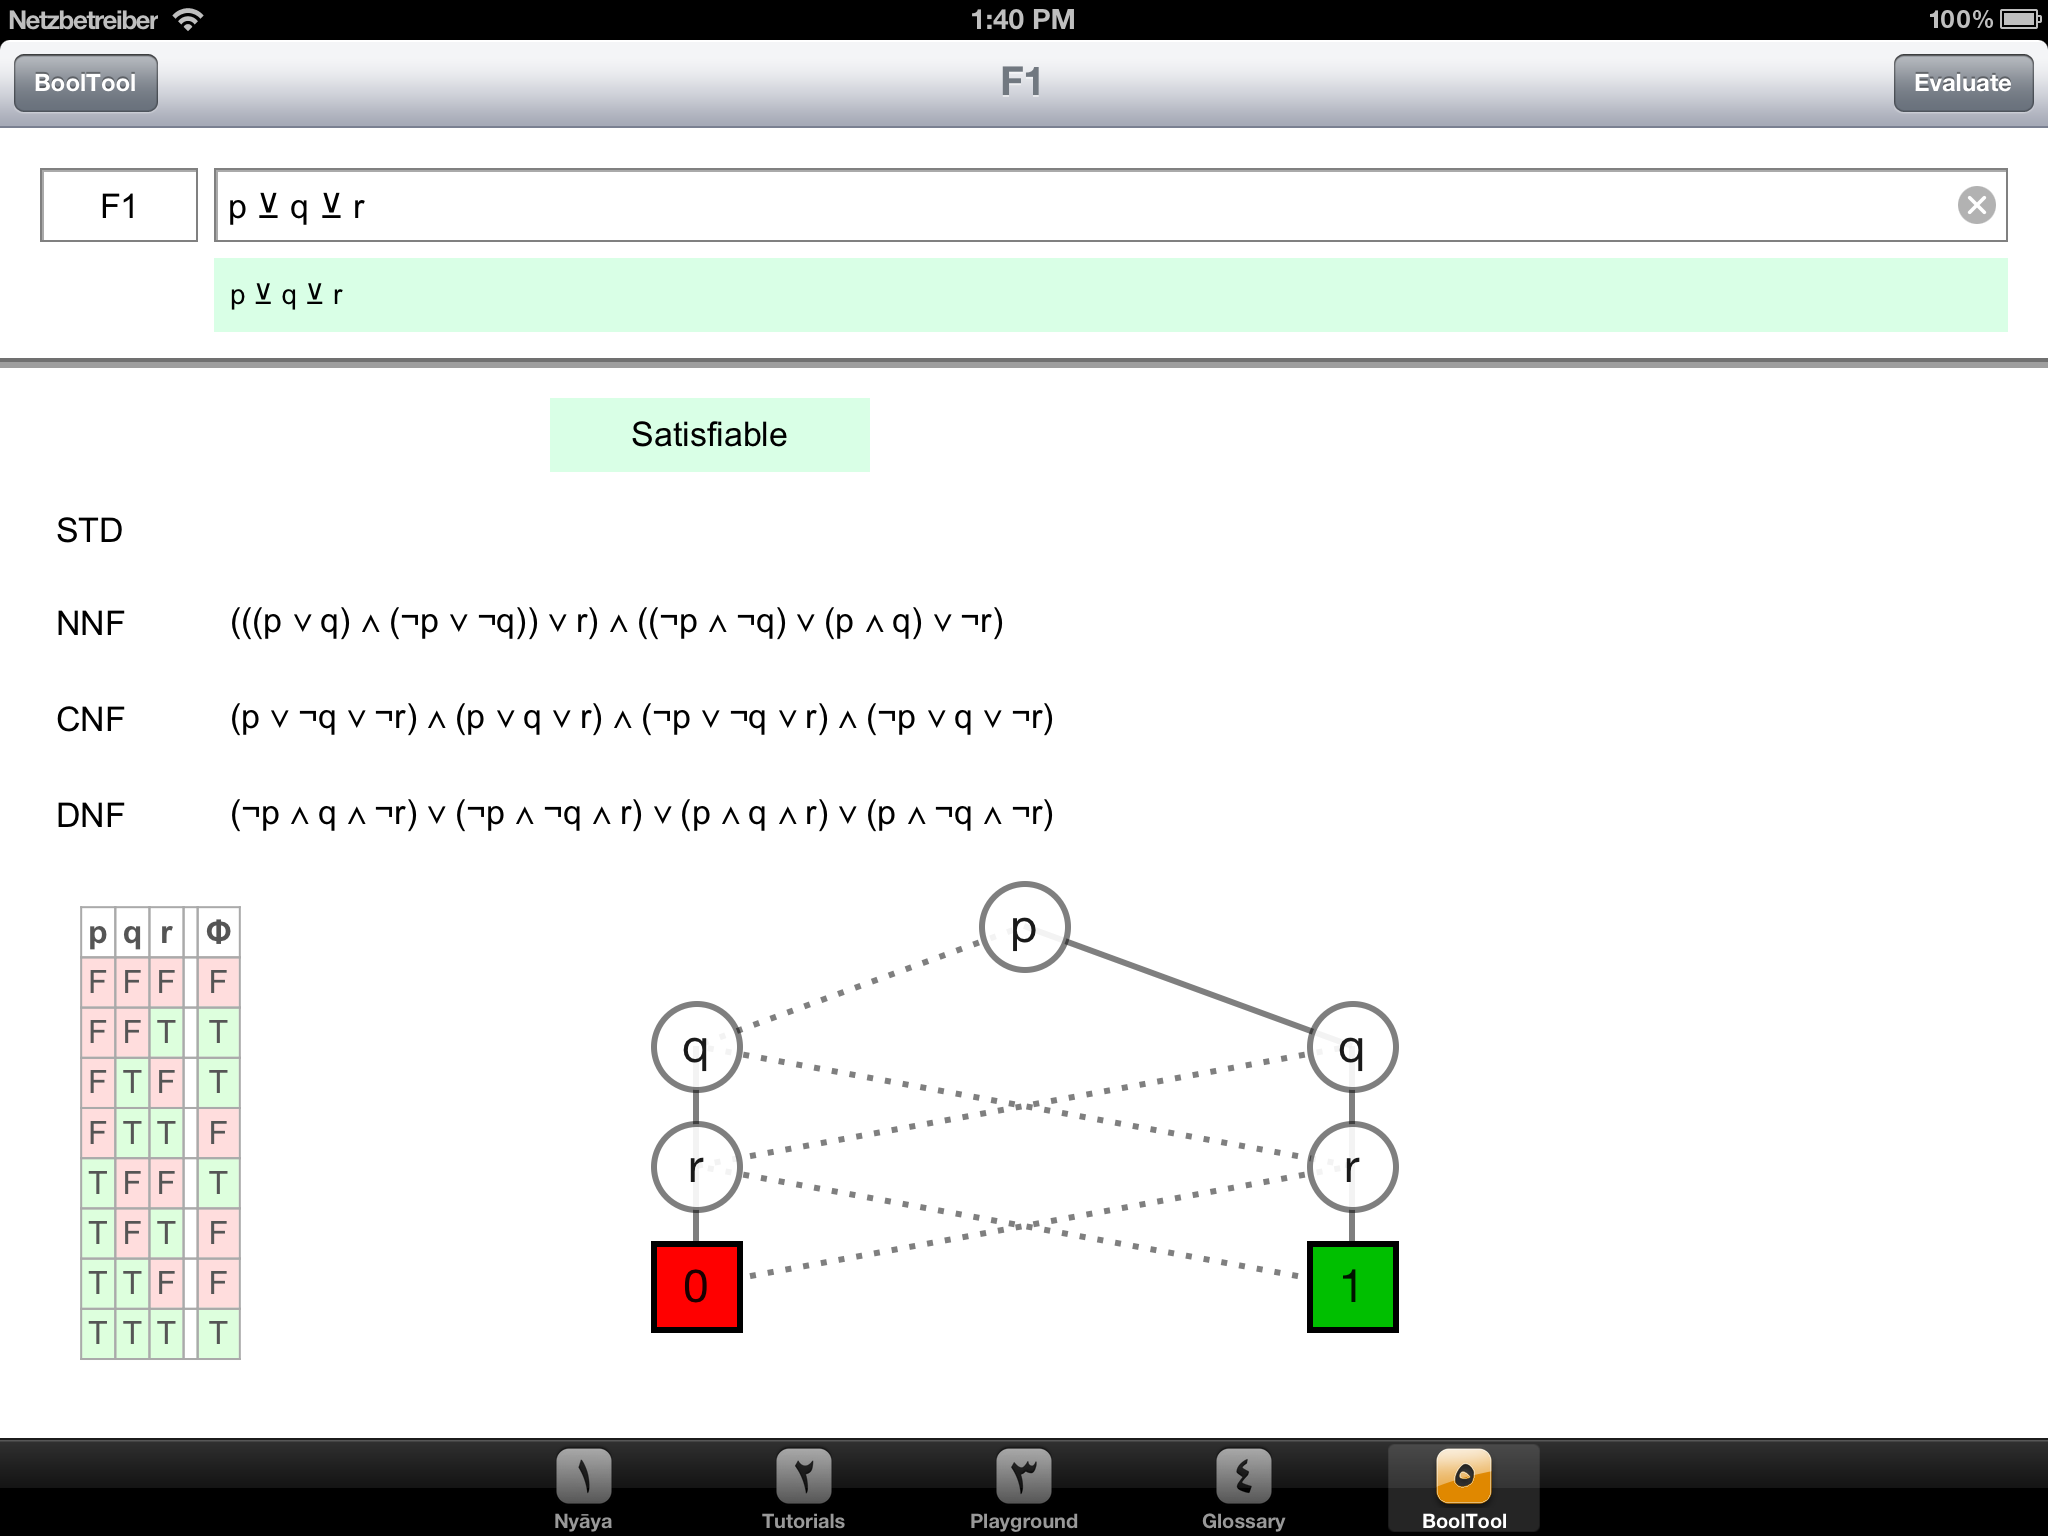
\includegraphics[width=13cm]{concept/BoolTool.png}
\caption{Boolean function $p \oplus q \oplus r$}
\label{fig:BoolToolOutput}
\end{center}
\end{figure}



